\documentclass{article}
\usepackage{graphicx}
\usepackage{hyperref}
\usepackage[margin=0.75in]{geometry}
\usepackage[utf8]{inputenc}
\usepackage{indentfirst}
\usepackage{amsmath,amssymb}

\DeclareRobustCommand{\bbone}{\text{\usefont{U}{bbold}{m}{n}}}

\DeclareMathOperator{\EX}{\mathbb{E}}% expected value


\setlength{\parindent}{4em}
\setlength{\parskip}{1em}
\renewcommand{\baselinestretch}{2.0}

\begin{document}
\title{BIOS 611 Project 1}
\author{Jane She \\ e-mail: jane.she@unc.edu}
\date{19 October 2021}
\maketitle

\section{Introduction}


Men's college basketball is a widely popular sport, especially at the Division 1 level and is broadcasted nationally for fans to watch. According to Cav's Corner, the UVA men's basketball team is one of the top revenue generators for the school. 

As a recent graduate of the University of Virginia, I was interested in looking at various game statistics and their infuences on the number of games won by a team. I specificially looked at the 2019 NCAA D1 basketball season since that is both the year that UVA won the national championships and the last pre-COVID season.

In this report, I examined the relationship between the number of games won and statistics including adjusted offensive efficiency, adjusted defensive efficiency, effective field goal percentage, turnover rate, and steal rate.

\section{Data}

The dataset with variable descriptions and more context can be found \href{https://www.kaggle.com/andrewsundberg/college-basketball-dataset}{here} and was found on kaggle. Originally, the data was scraped from barttorvik.com, a famous college basketball website. 

\section{Exploratory Data Analysis}

In our exploratory data analysis, I decided to choose a couple variables I was interested in and plot them against the number of wins. The variables I included are adjusted offensive efficiency, adjusted defensive efficiency, effective field goal percentage shot, turnover rate, and steal rate.

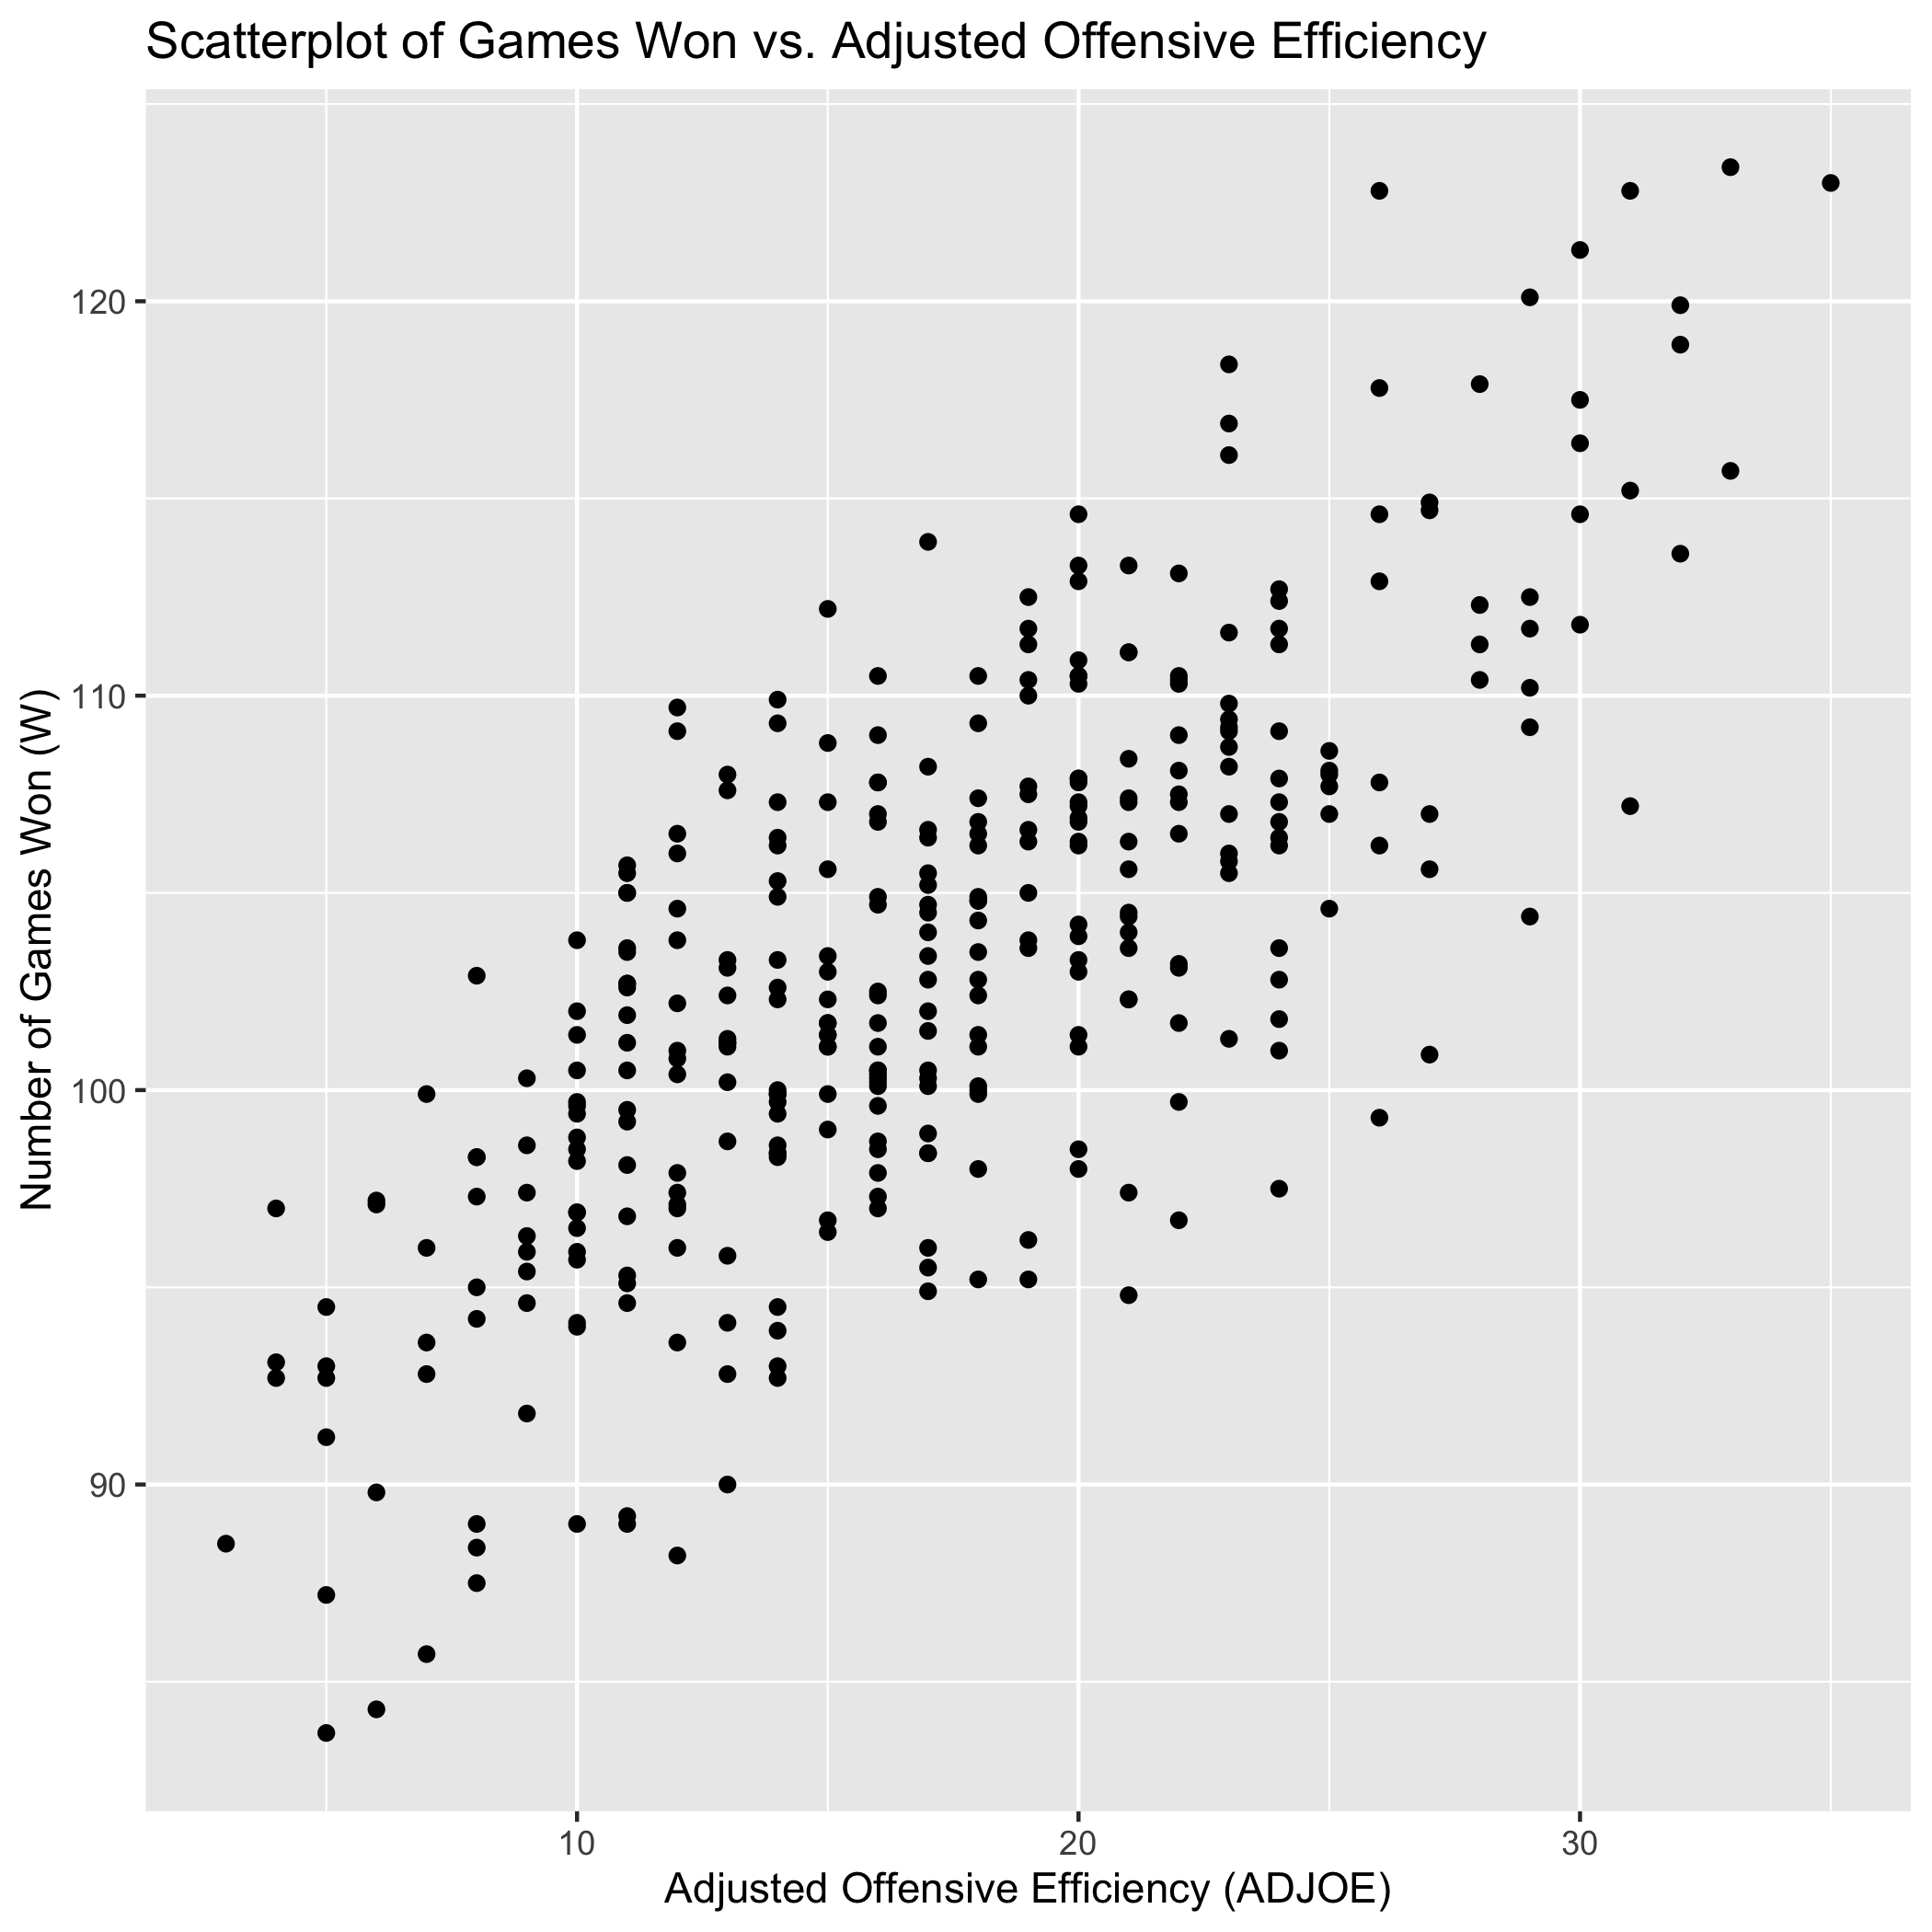
\includegraphics[width=0.5\textwidth]{Figures/W_ADJOE.png}\\
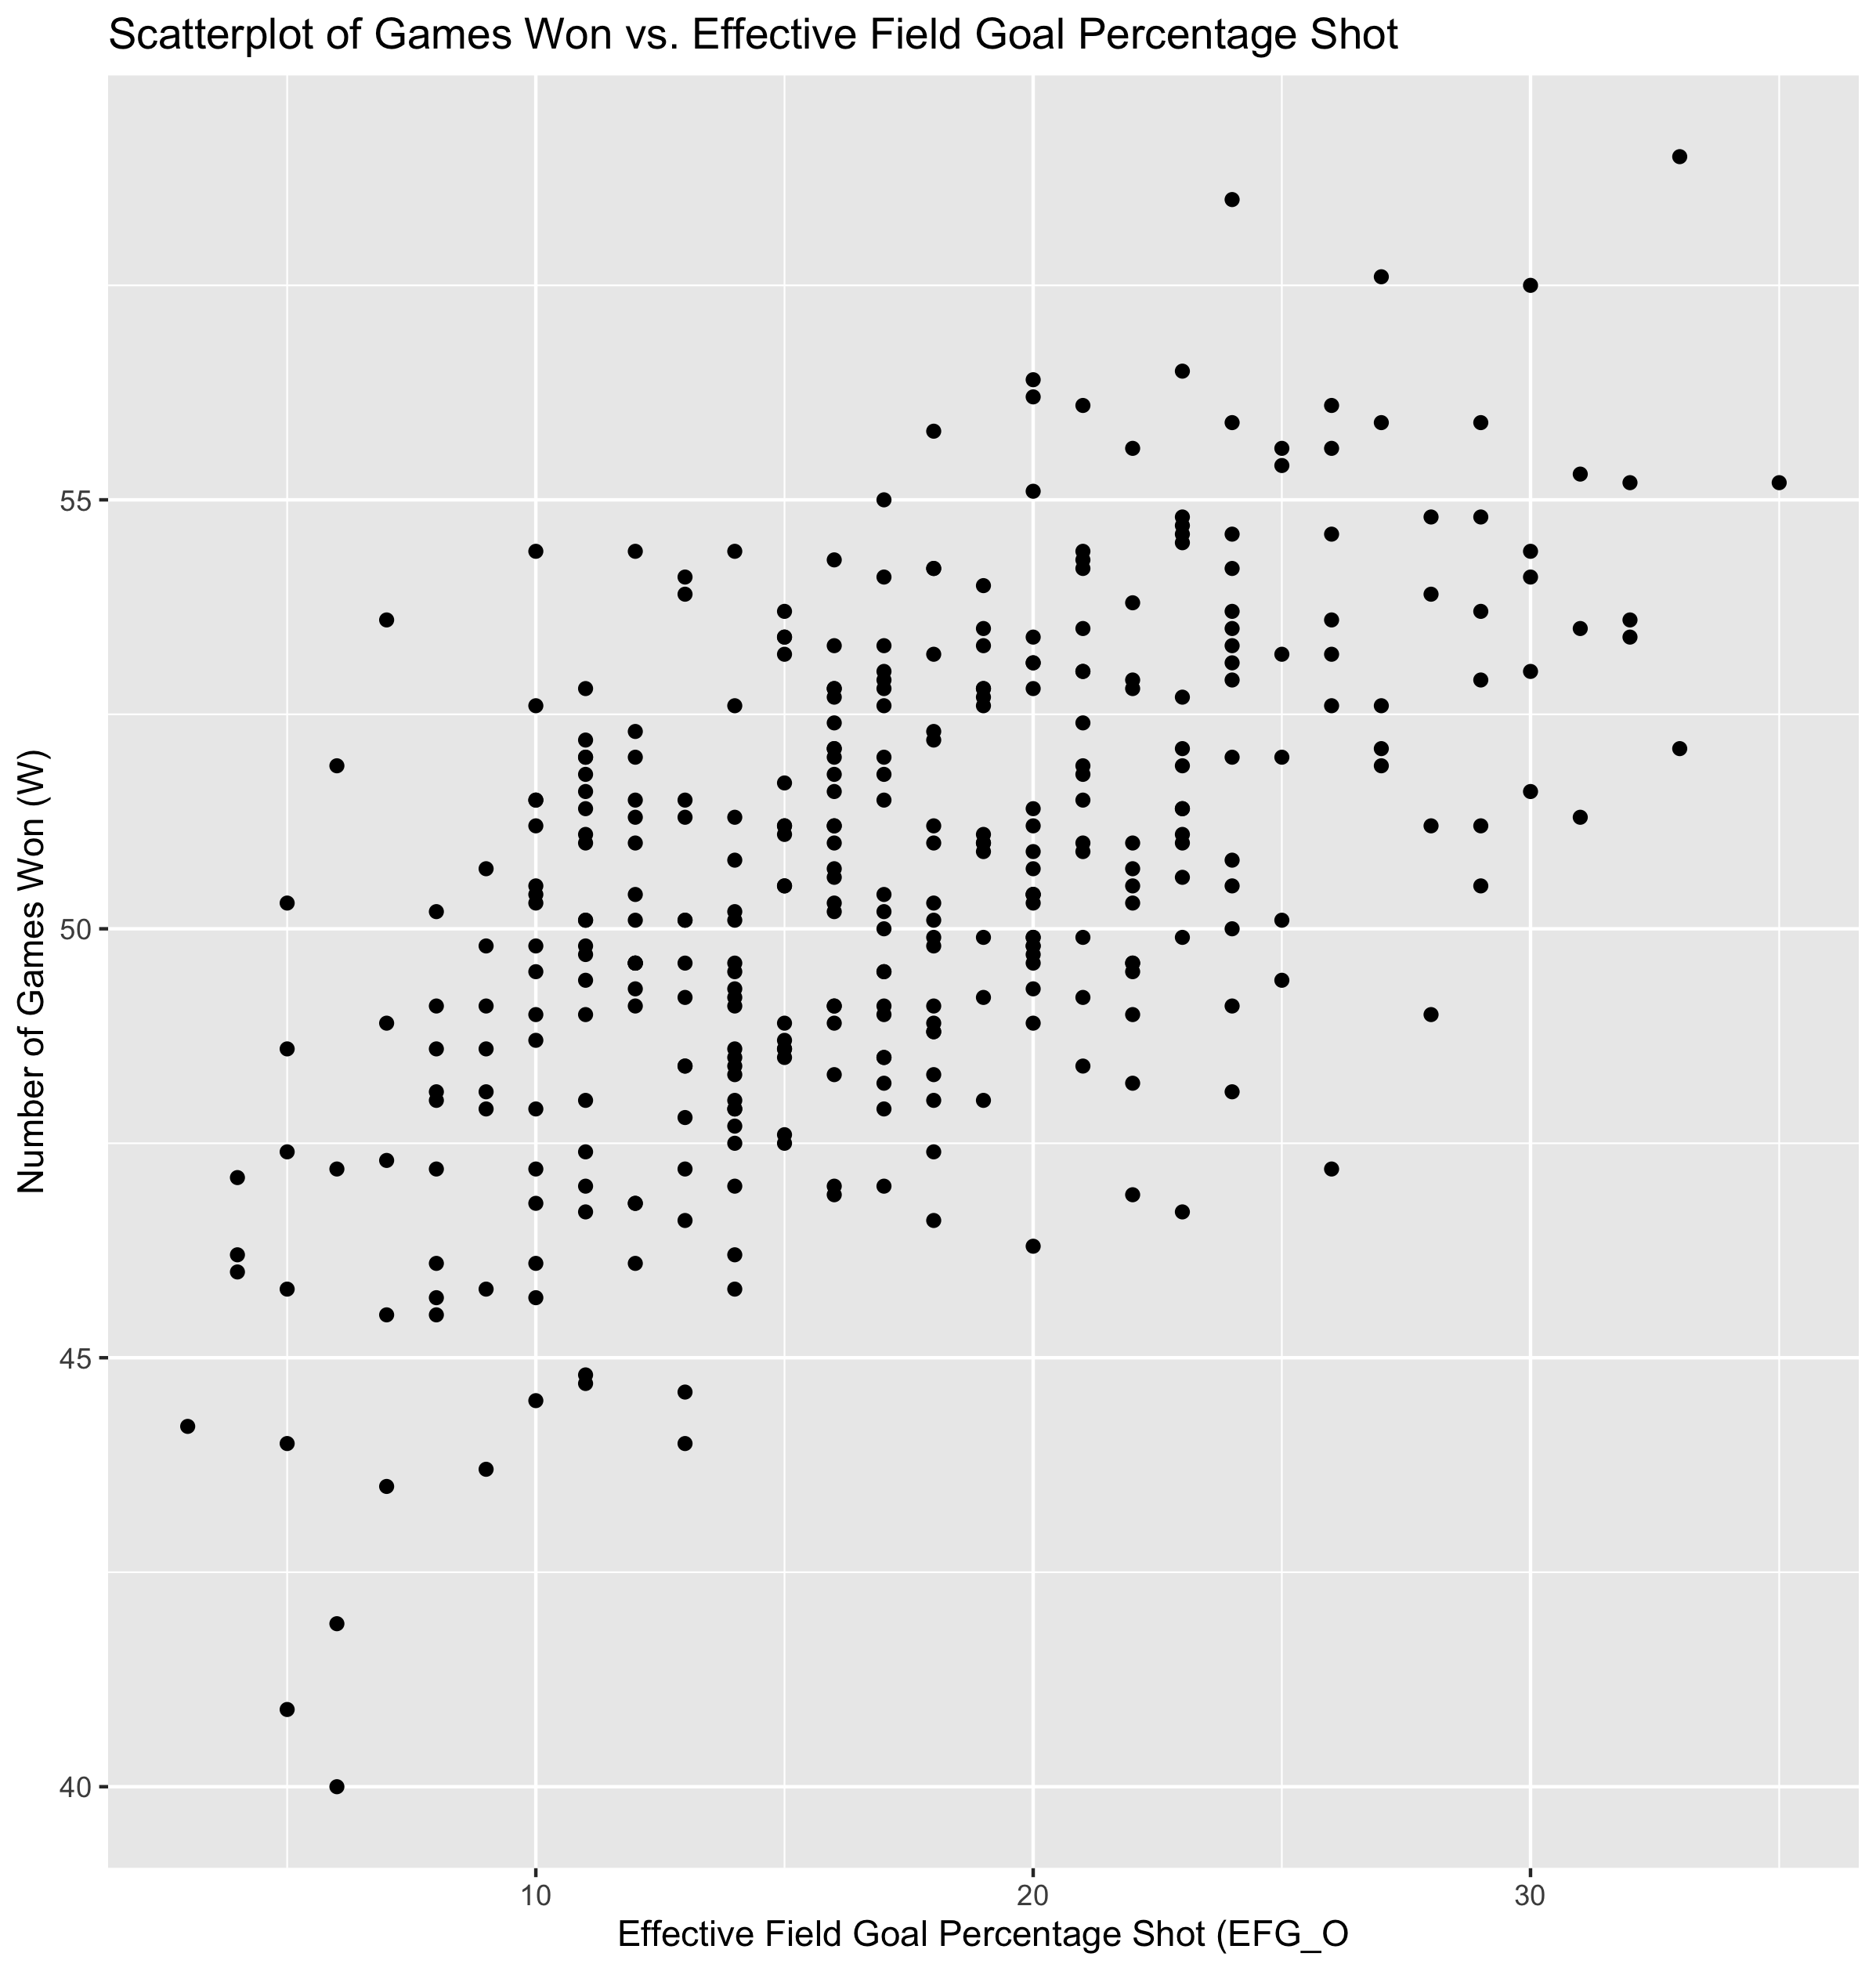
\includegraphics[width=0.5\textwidth]{Figures/W_EFGO.png}\\
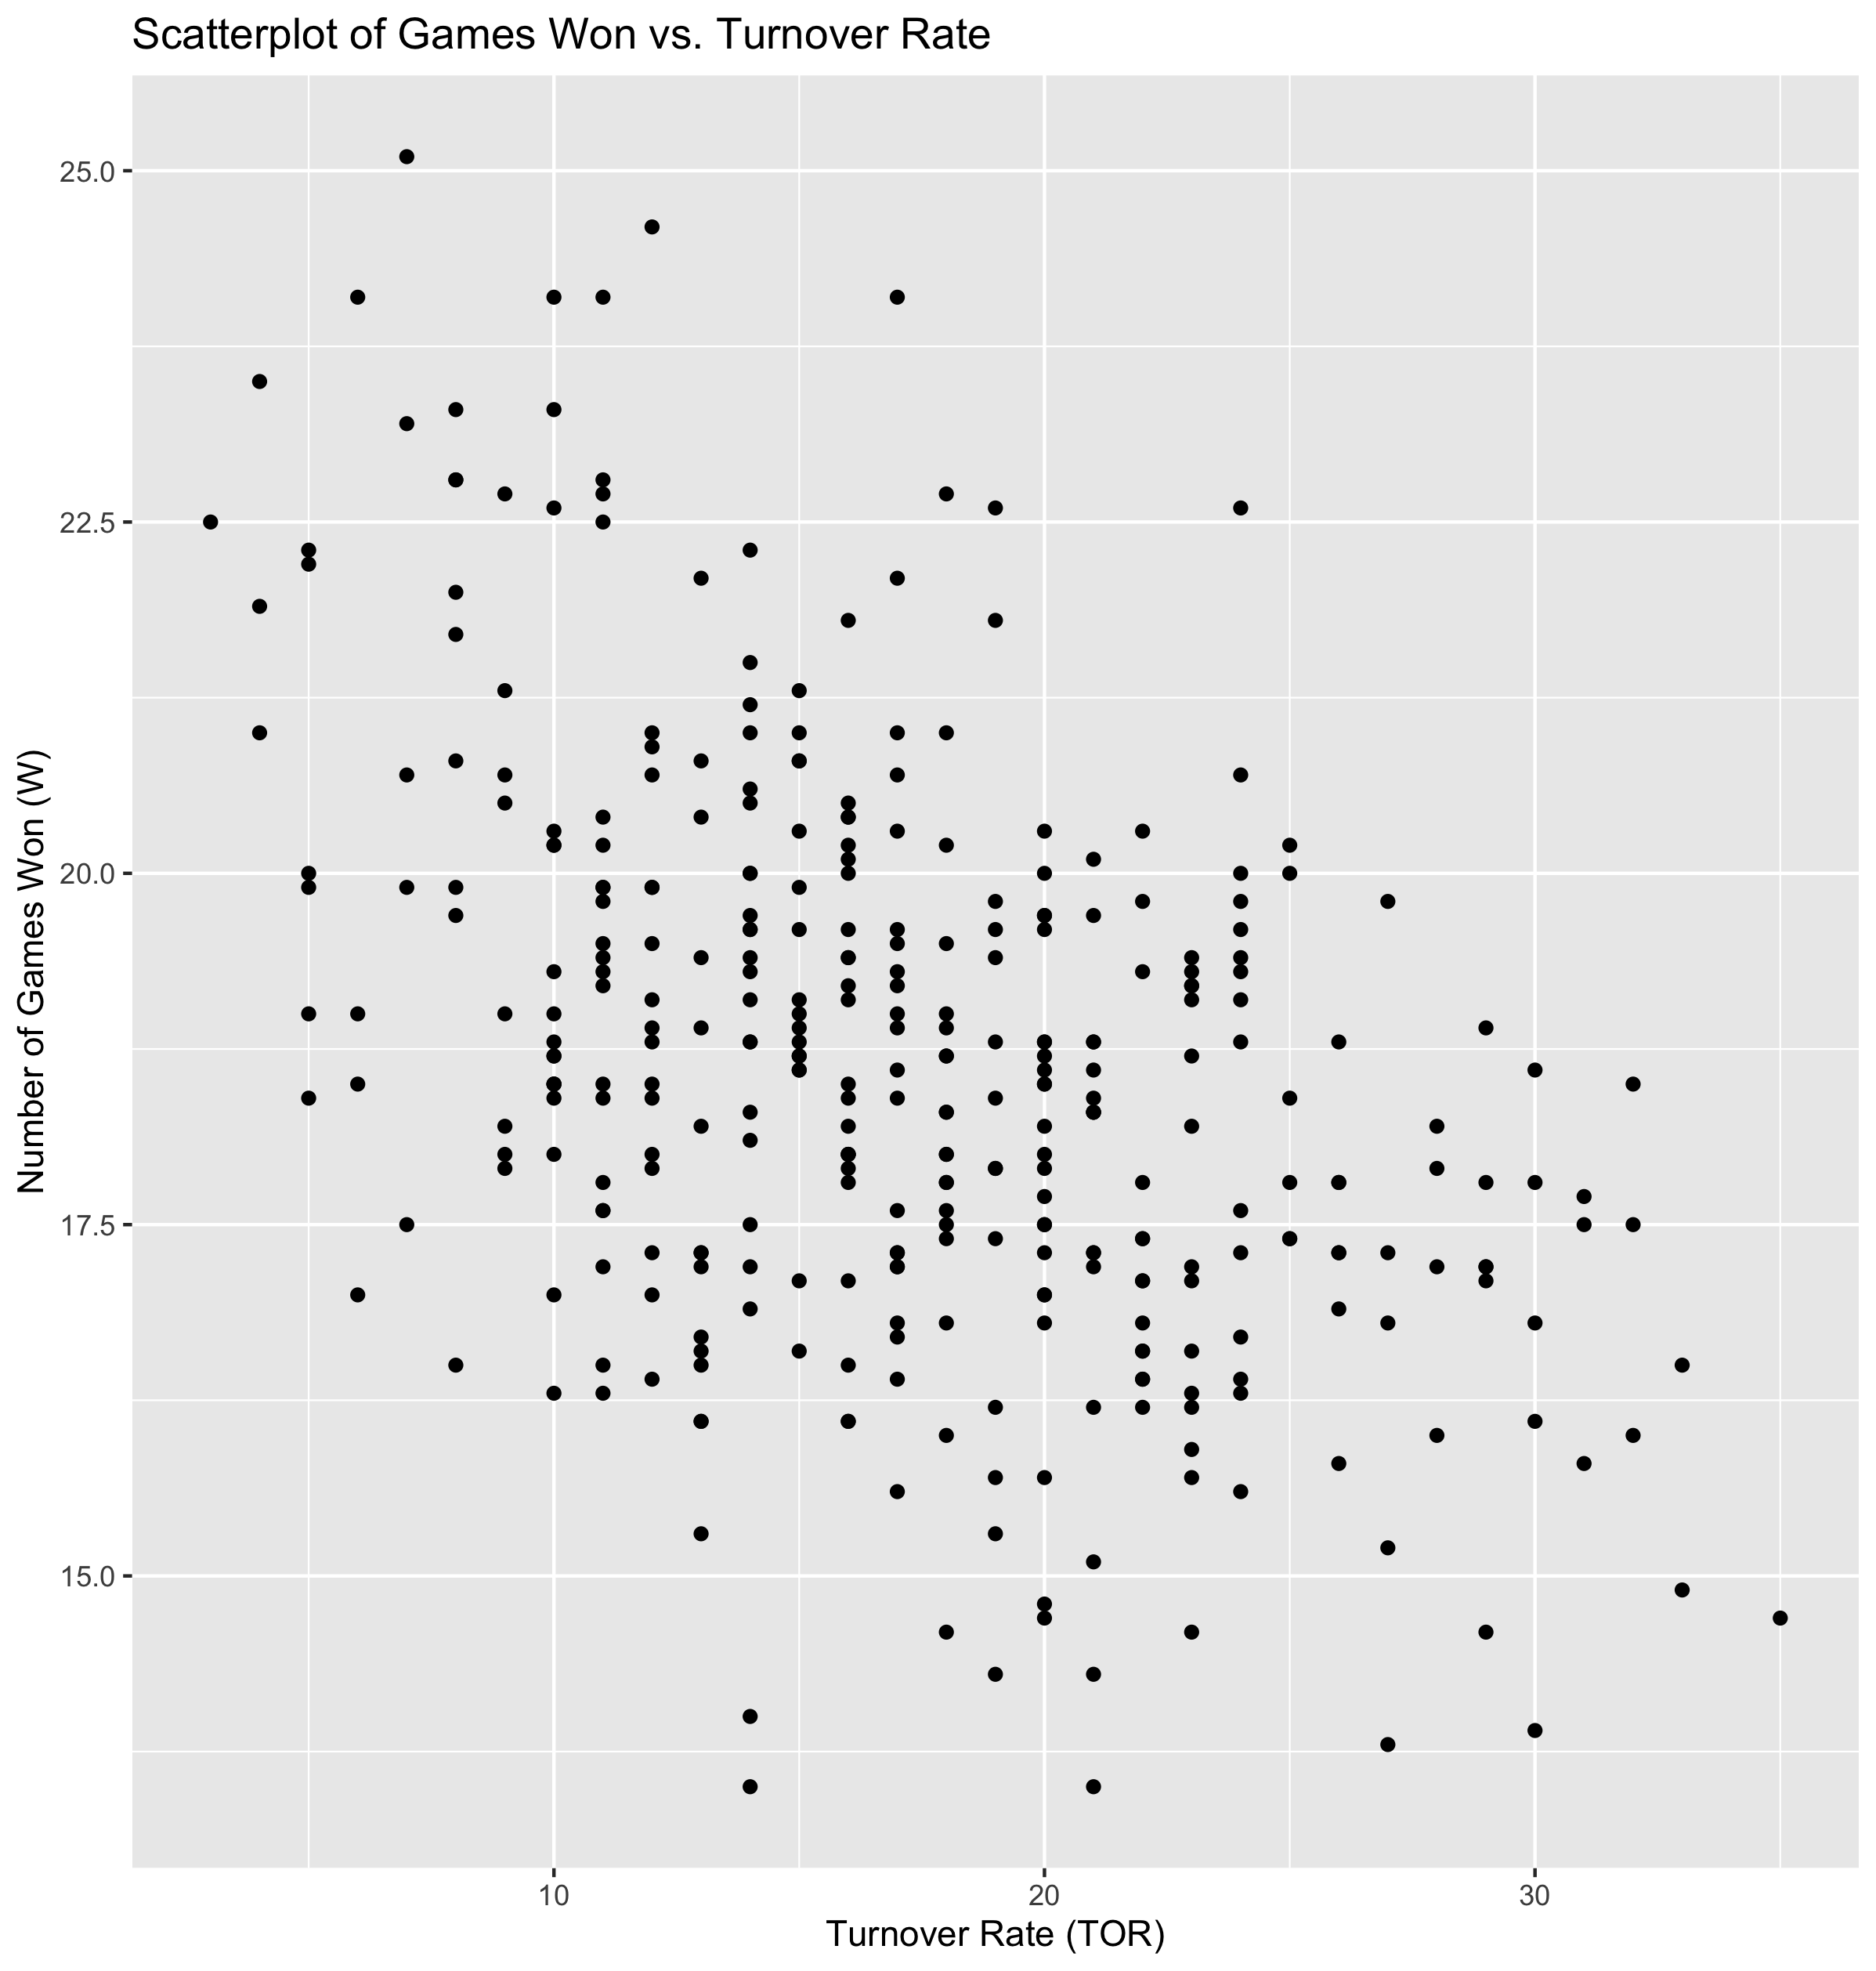
\includegraphics[width=0.5\textwidth]{Figures/W_TOR.png}\\
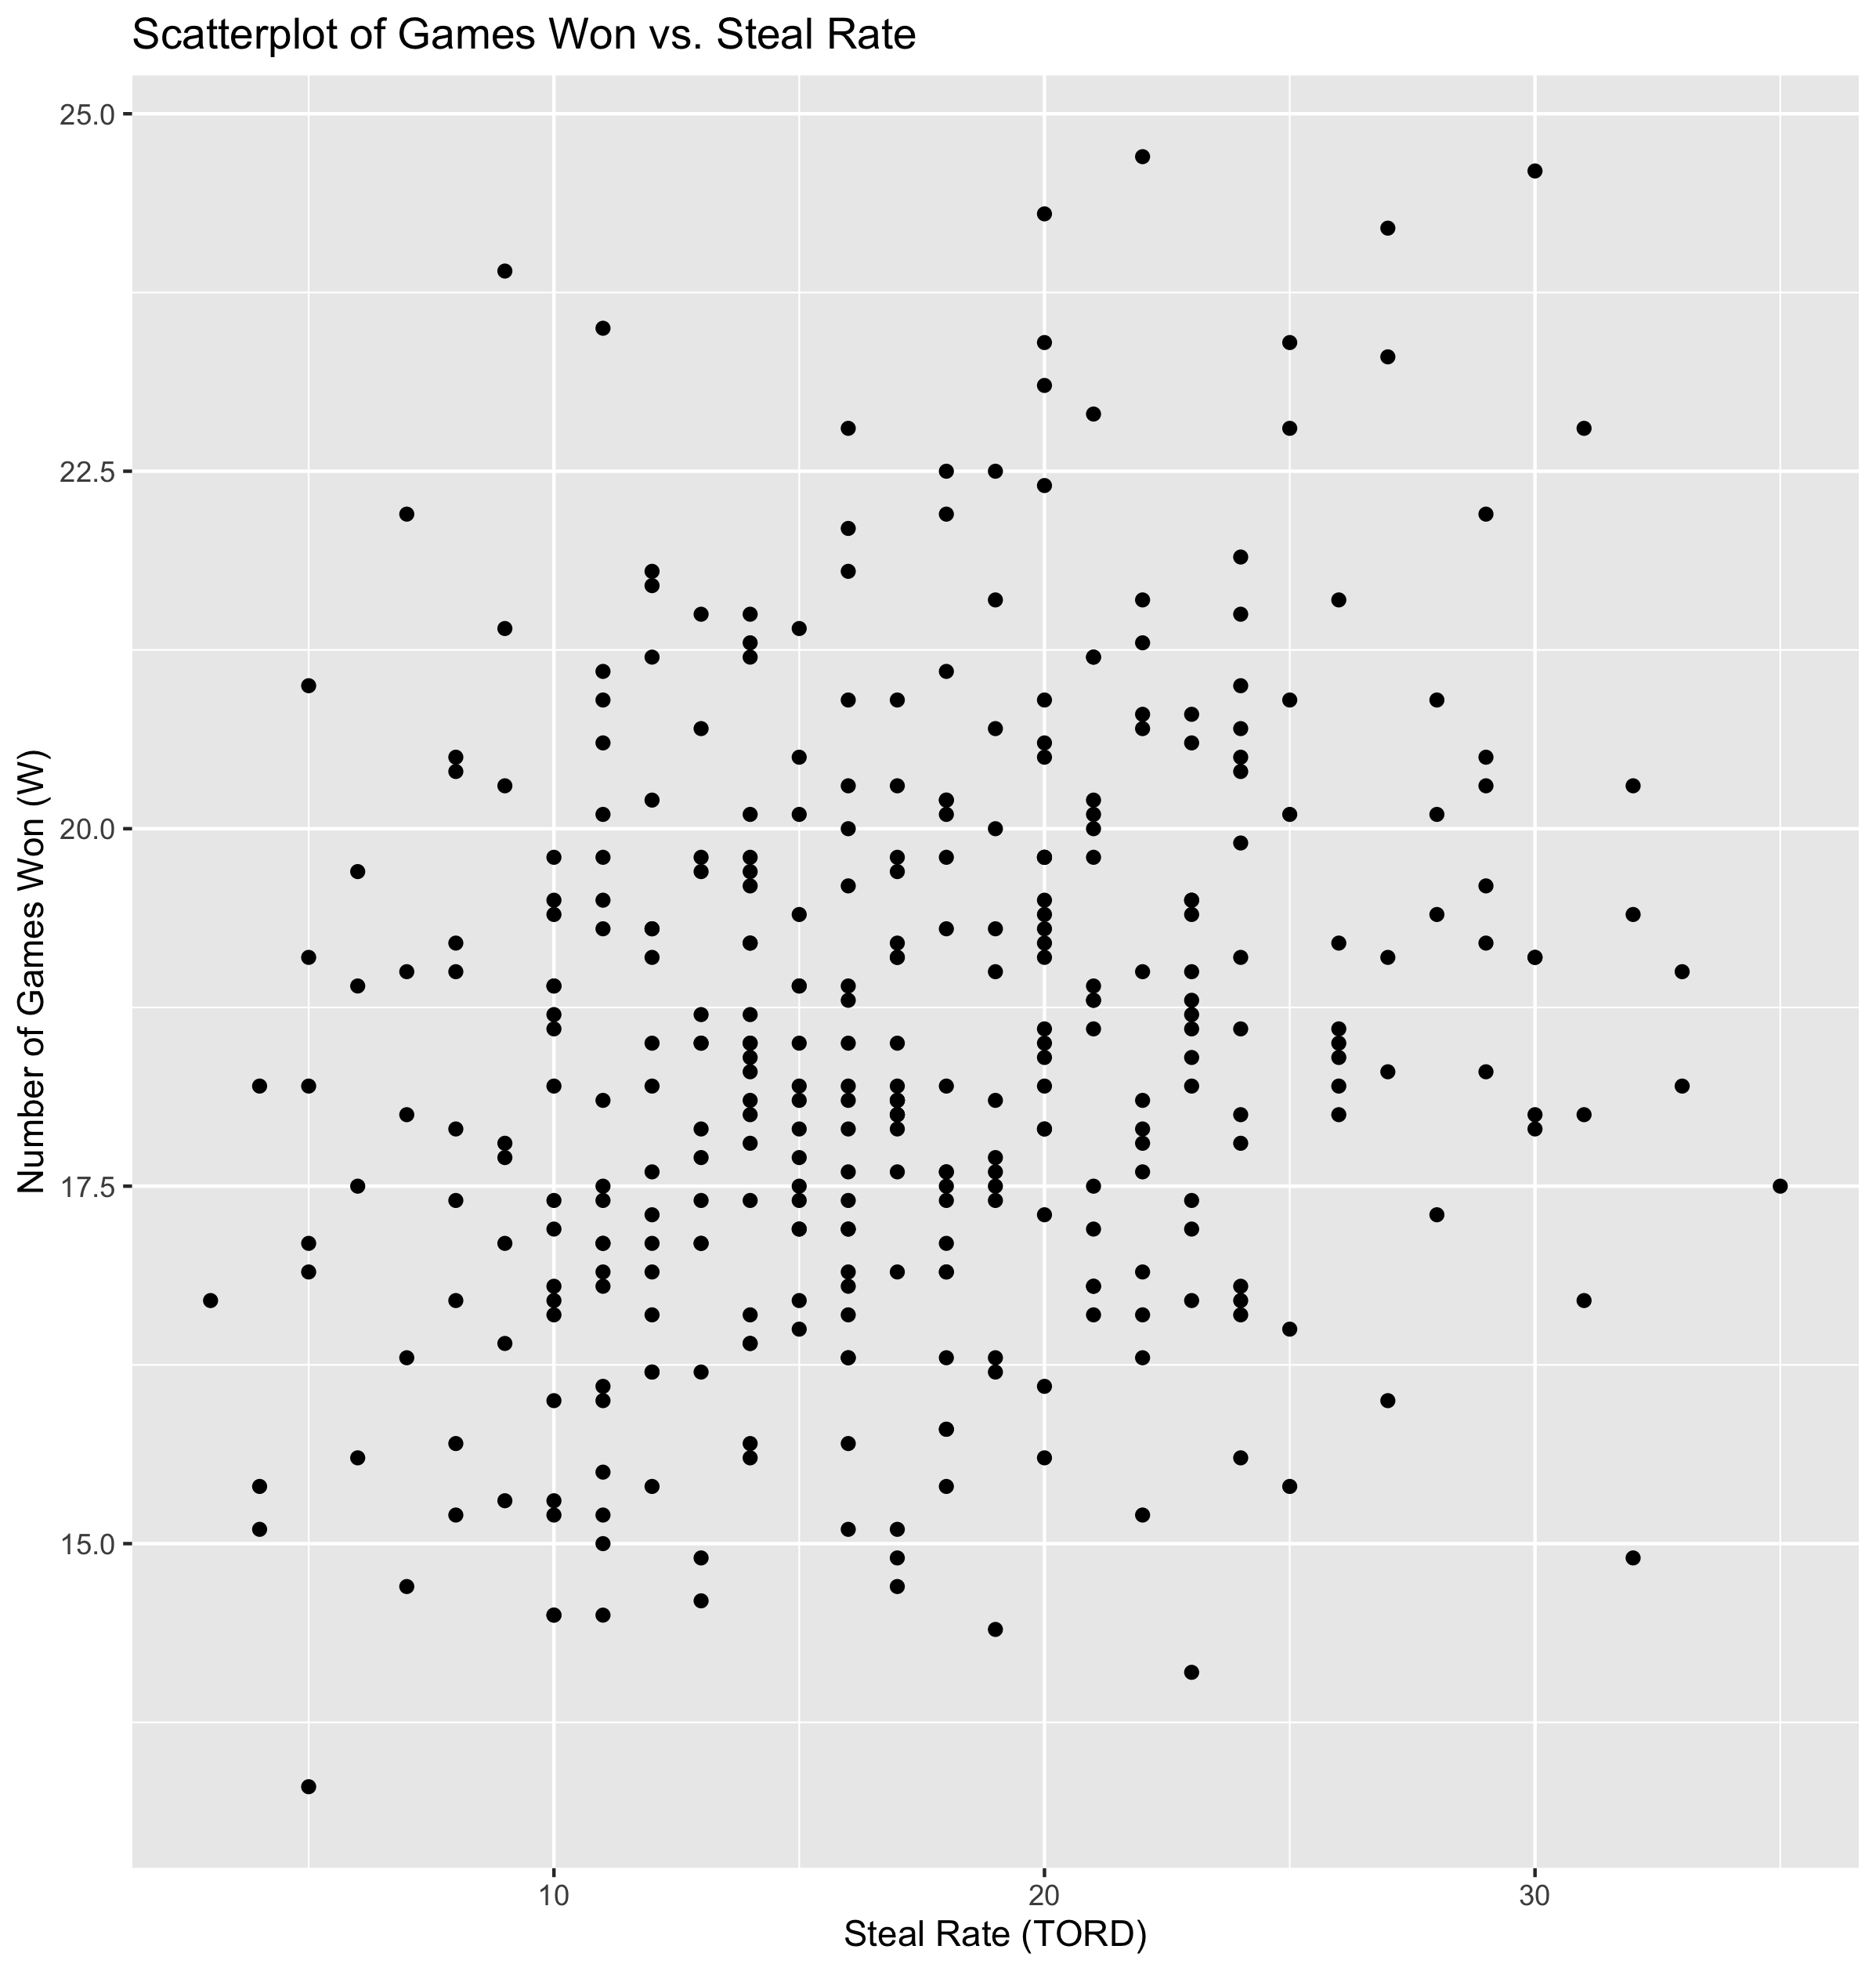
\includegraphics[width=0.5\textwidth]{Figures/W_TORD.png}\\

Additionally, I created a correlation matrix along with a graph of some pairwise interactions.

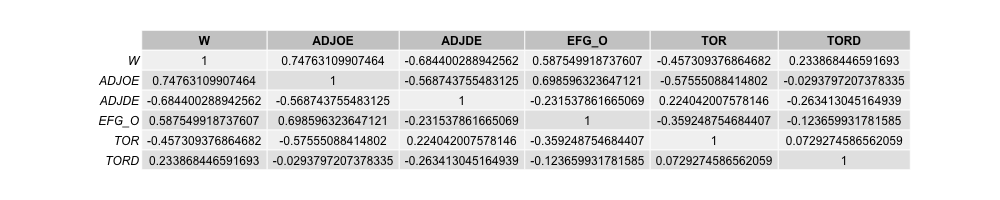
\includegraphics[width=0.8\textwidth]{Figures/correlation_matrix.png}\\

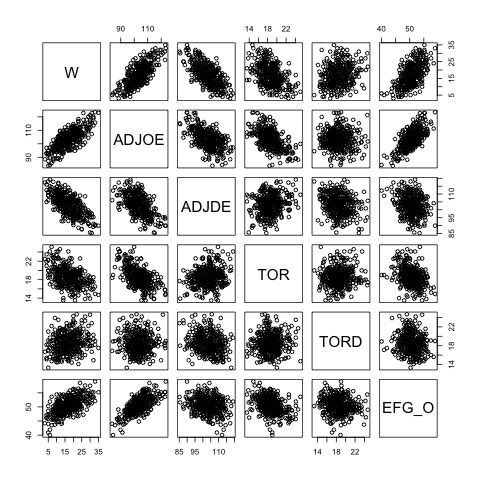
\includegraphics[width=0.8\textwidth]{Figures/pairwise_interaction.png}\\


\section{Analysis- Model Building}

During model building, I started off using only a couple quantitative predictors that looked like they had the strongest linear relationships from the EDA to predict the number of games won which include both the regular season and post-season. The three quantitative predictors I chose to use were ADJOE, ADJDE, and EFGO.

\subsubsection*{First Stage Model}

Our first stage hypothesized model was: 

\begin{itemize}

  \item $\mathbb{E}(Games Won) = \beta_{0} + \beta_{1}(ADJOE) + \beta_{2}(ADJDE) + \beta_{3}(EFGO)$ 
  
\end{itemize}


After conducting an F-test, we returned an F test statistic of 263.14 with a significant p-value. Meaning, this first model is adequate for predicting the number of games won. 

\subsubsection*{Qualitative Predictors}

Next, I added some qualitative predictors by turning the variable, WAB $(wins-above-bubble)$ into levels by certain bins. There were a total of 5 bins with equal lengths to be used as a categorical variable.

The bubble refers to the cut-off between making the NCAA March Madness Tournament and not making it. 

These bins along with their dummy coding were:

Base level: -23.2:-16:48

X1: x1 = 1 if [-16.48, -9.56), x1 = 0 if not

X2: x2 = 1 if [-9.56, -2.64), x2 = 0 if not

X3: x3 = 1 if [-2.64, 4.28), x3 = 0 if not

X4: x4 = 1 if [4.28, 11.2), x4 = 0 if not

Our second stage hypothesized model with the dummy variables was:

\begin{itemize}

  \item $\mathbb{E}(Games Won) = \beta_{0} + \beta_{1}(ADJOE) + \beta_{2}(ADJDE) + \beta_{3}(EFGO) + \beta_{4}(x1) + \beta_{5}(x2) + \beta_{6}(x3) + \beta_{7}(x4)$ 
  
\end{itemize}

Since our F test was significant, our second model with qualitative predictors is adequate for predicting games won. 

\subsubsection*{Adding Interaction}

An interaction I thought could be important was WAB*ADJOE since I believed that the more points a team scores, the more likely they may be to make the March Madness tournament. 

My third stage hypothesized model included the interaction between WAB and ADJOE which also returned a significant result from a global F-test and thus is adequate for predicting games won. 


\begin{itemize}

  \item $\mathbb{E}(Games Won) = \beta_{0} + \beta_{1}(ADJOE) + \beta_{2}(ADJDE) + \beta_{3}(EFGO) + \beta_{4}(x1) + \beta_{5}(x2) + \beta_{6}(x3) + \beta_{7}(x4) + \beta_{8}(ADJOE*x1) + \beta_{9}(ADJOE * x2) + \beta_{10}(ADJOE * x3) + \beta_{11}(ADJOE *x4)$ 
  
\end{itemize}


\subsubsection*{Evaluating Interaction}

Although the complete model which included interaction terms was significant, it may not neccessarily be better than our second stage model. Thus, I wanted to evaluate if adding the interaction bettween WAB*ADJOE was actually significant or not.

I performed a nested F-test comparing my complete model with my reduced model:

\begin{itemize}

  \item COMPLETE: $\mathbb{E}(Games Won) = \beta_{0} + \beta_{1}(ADJOE) + \beta_{2}(ADJDE) + \beta_{3}(EFGO) + \beta_{4}(x1) + \beta_{5}(x2) + \beta_{6}(x3) + \beta_{7}(x4) + \beta_{8}(ADJOE*x1) + \beta_{9}(ADJOE * x2) + \beta_{10}(ADJOE * x3) + \beta_{11}(ADJOE *x4)$ 

  \item REDUCED: $\mathbb{E}(Games Won) = \beta_{0} + \beta_{1}(ADJOE) + \beta_{2}(ADJDE) + \beta_{3}(EFGO) + \beta_{4}(x1) + \beta_{5}(x2) + \beta_{6}(x3) + \beta_{7}(x4)$ 
  
\end{itemize}

Our result returned a significant p-value which implies that our parameters are significantly different from 0, and that the interaction between WAB*ADJOE is significant. Our complete model is better than our reduced model. Which leaves us with our final model as the "Complete" model above. 

\section{Checking Model Assumptions}

The assumption that the mean of our error term $\epsilon$ held true from our residual plot since we don't see any patterns in the Residuals vs. Fitted graph.

Our scale location plot is approximately horizontal with pretty much even spread around it, which means our assumption of constant variance is met. 

To check our normality assumption, we can look at our QQ plot. Our line approximately follows the dashed diagonal line. However, the front and the tail of the data seem to deviate a little. 

We can also see that we have several influential observations with a couple of outliers. 

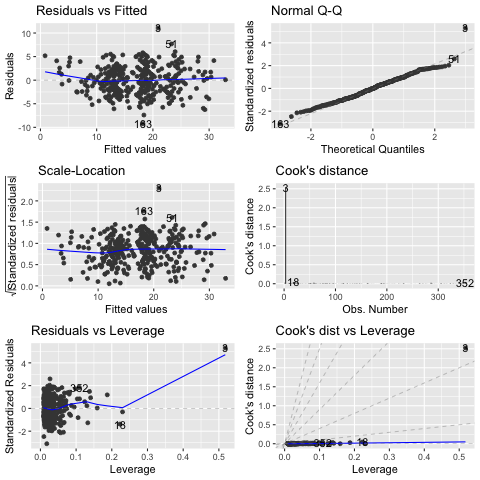
\includegraphics[width=0.8\textwidth]{Figures/model_assumptions.png}\\



\end{document}
